
\chapter{Physics PGR conference and Annual Progress Monitoring (20/04/2017)}

Every year, a postgraduate researchers conference is held where students demonstrate what they've been doing so far. First year PGRs are tasked to make a poster detailing their projects, stand next to it for certain amount of time, and explain things and answer questions to people who view it. This year's conference is on 10\textsuperscript{th} May. My poster (actual size is A0) is displayed below.

\section{Annual Progress Monitoring (07/06/2017)}

Annual Progress Monitoring is used to ensure that PhD students have made sufficient progress to move forward to the following year. For first year students, a report has to be written detailing the progress made over the year, as well as future plans. A presentation to the HEP group must also be made (in my case). My report and presentation are linked here: \href{run:modules/Sec 22 - Physics PGR conference and Annual Progress Monitoring/figures/FirstYearReport.pdf}{First Year Report} and \href{run:modules/Sec 22 - Physics PGR conference and Annual Progress Monitoring/figures/20170607 Presentation to HEP group (07-06-2017)/Presentation to HEP group.pdf}{First Year Presentation}.

From the viva/interview, there were several comments and aspects I need to take into account.

\begin{easylist}[itemize]
\easylistprops
& I need to know the entire process of DM production from the protons (and partons) within the beam, to how they interact and produce the particles (including sparticles), to the specifics of the analysis.

& That we use \emph{transverse} energy and momentum because -- for, e.g., SUSY production -- quark-antiquark annihilation is the predominant collision. Then most of decay products are jets because QCD is the favoured interaction; it's called the "strong" force for a reason. And you don't know the exact longitudinal momentum of the partons, but we know that the transverse momentum before the collision (which has to equal the momentum after) is zero because the protons are travelling completely longitudinally. The beams have equal and opposite momentum but that doesn't hold for the individual partons within each proton in the beam. Quarks tend to have a greater proportion of the momentum over the antiquarks (because protons are predominantly matter, not antimatter), which the Parton Distribution Functions show. The normalisation of PDFs require that the valence quantum numbers for a particle are reproduced. So for a proton, the integral over the total momentum of the difference in probability of a $u$ carrying a certain momentum and a $\bar{u}$ carrying an equal momentum yields 2 (the number of valence $u$s in the proton). So, if $f_q(x)$ is the probability of a quark flavour $q$ carrying a momentum fraction $x$ of the proton's longitudinal momentum,

\begin{equation}
\int^1_0 dx( f_u(x) - f_{\bar{u}} ) = 2
\end{equation}

as described in slide 6 of \url{https://www2.physics.ox.ac.uk/sites/default/files/2014-03-31/qcdgrad_rojo_oxford_tt14_5_dis_pdf_19197.pdf} or section 2 of~\cite{Pennington:2016dpj}.

The Higgs is normally produced from gluon-gluon fusion (with a triangle of, normally, top quarks that decays into the Higgs). But that doesn't work for SUSY particles because the gluons don't usually have enough energy to produce these particles, so it's $q\bar{q}$ for the most part.

& The unique thing about RA1 is the use of \alphat. It cuts QCD heavily by constraining jet imbalance, so removes a lot of potential "fake MET" from misreconstructed jets. The figure below (from~\cite{CMS-PAPER-SUS-15-005-arXiv}) shows that QCD-driven final states drop sharply at around $\alphat = 0.5$, and so we tend to make cuts a little higher than this value to reduce the QCD background to a much lower level. This allows a cleaner search for SUSY by using MET as a variable. We're sensitive to strongly-coupled SUSY. The use of \biasedDPhi\ greatly reduces QCD as well, with the reference above containing a corresponding plot of the events vs \biasedDPhi.

\begin{figure}[htbp]
\centering
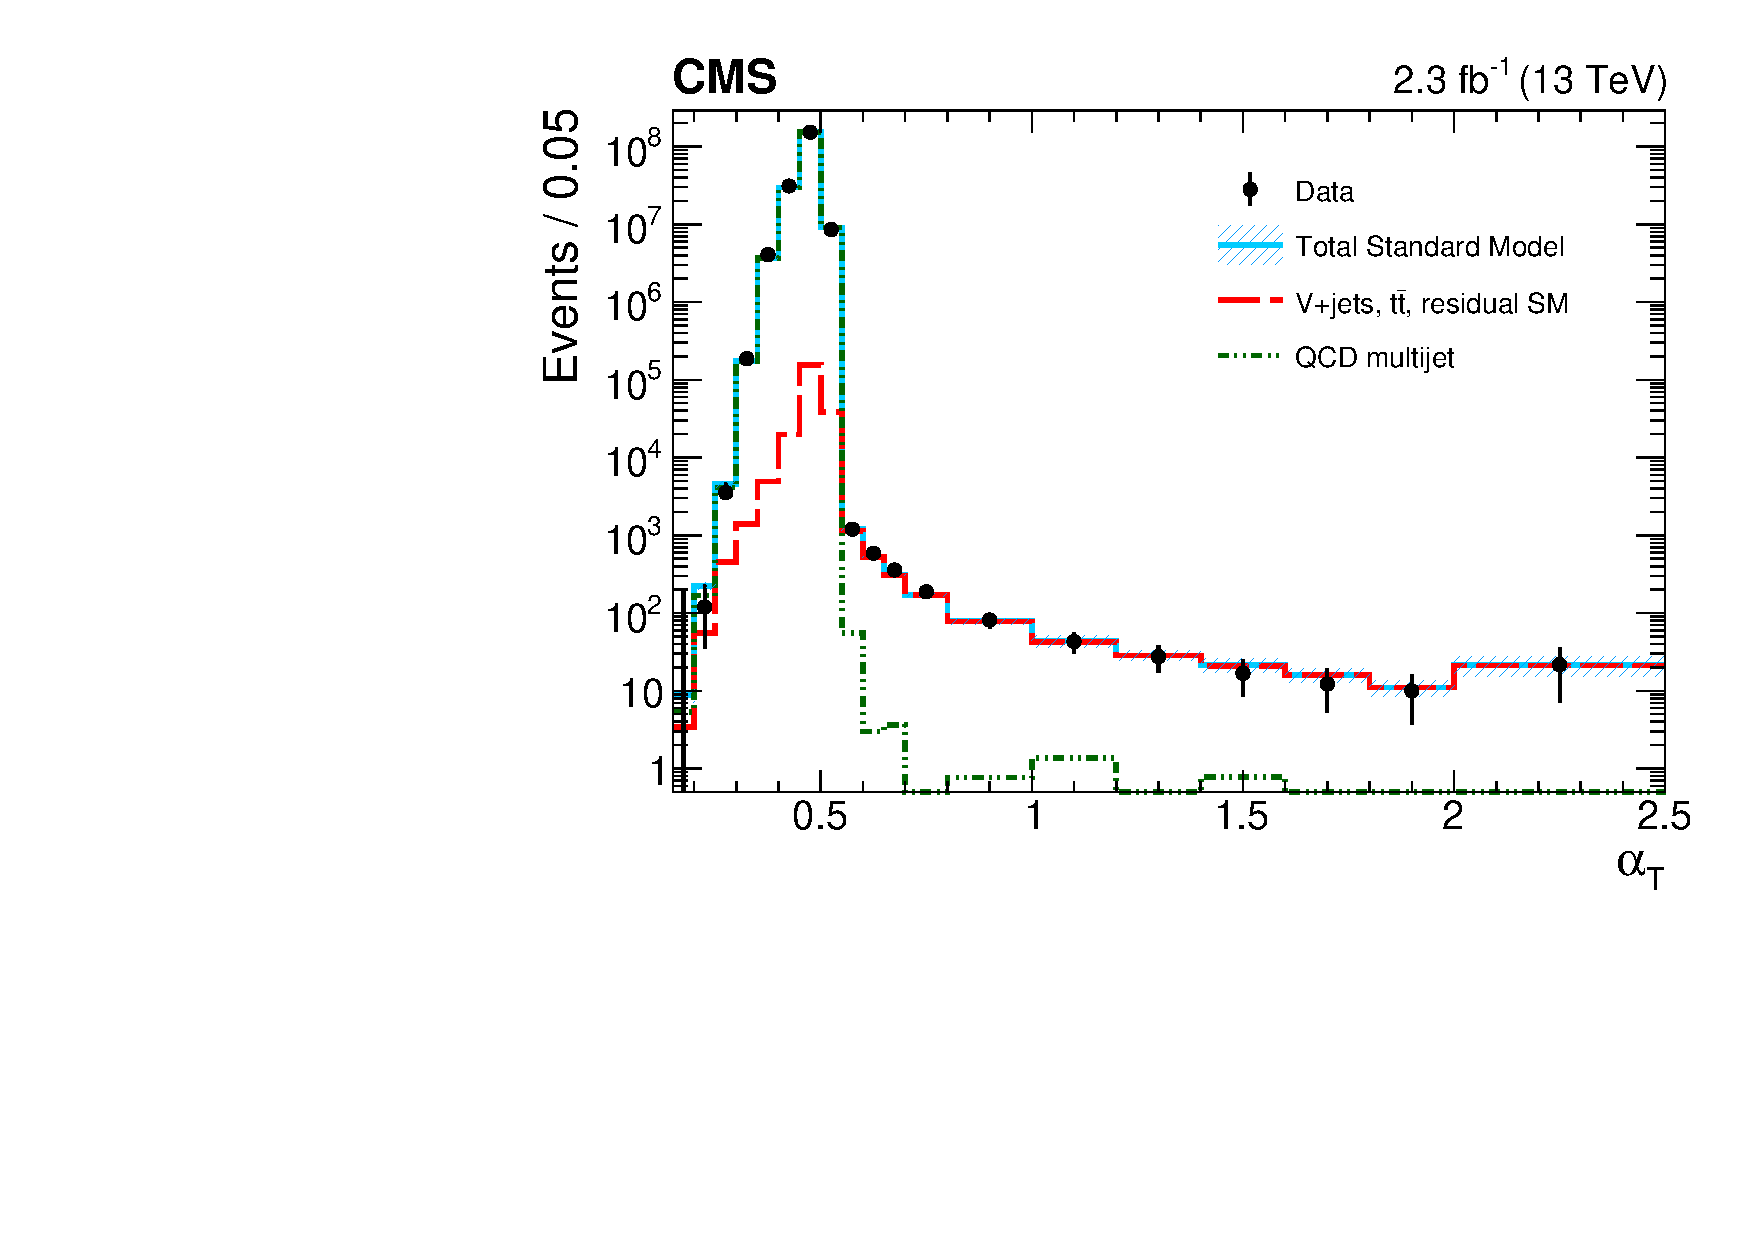
\includegraphics[width=\textwidth]{figures/CMS-SUS-15-005_Figure_001-a.pdf}
\caption{The \alphat\ distribution observed in data for events that satisfy the selection criteria defined in the text. The statistical uncertainties for the multijet and SM expectations are represented by the hatched areas (visible only for statistically limited bins). The final bin of the distribution contains the overflow events. }
\end{figure}

& RA1 looks at all hadronic final states because of the SUSY models we use. The gluinos and squarks decay into quarks, hence lots of jets and the need for \alphat. We use "natural" SUSY models because of the minimal fine-tuning of the bare Higgs mass that only need the gluino, third-generation squarks (stop and sbottom) and a Higgs-like LSP around the electroweak scale. These models are motivated by the discovery of a light Higgs boson.

& Need to research how the reference jets (GenJets) for JECs are made. Broadly, some people make unbiased Monte Carlo jets (i.e., before trigger cuts) that the L1 jets can be calibrated to. After some research, I've found some good descriptions in~\cite{Brooke:1602168}.

& That I should get more involved with the Trigger in the future. I'll pass on the JEC stuff to a younger student (like Joe has done to me) and get more involved in the development and stuff. It's also helpful that Bristol is so involved in the Trigger.

& My language is a little "loose" in the report. Need to take into account that I'm in a field where statements need to be very precise, as people scrutinise them, and English may not be the native language of some of the readers, so can misinterpret what I mean. So, things like the first sentence can be tightened up.

& At some point, I need to talk to Bjoern and Henning about how their supervisory roles are going to change because of Bjoern leaving. Presumably, Henning will become more involved with what I'm doing while Bjoern steps back a bit.

& Overall, Dave (Newbold) and Jonas were quite happy with how I've progressed so far, and have "high hopes for someone of your ability", and am "someone who can make a career out of this". I've been doing "pretty bloody well" according to Dave. They're happy that I've gotten quite involved in the analysis side of things and with the trigger.

\end{easylist}

If I want to read the interviewer and supervisor's comments (as well as my own), I can do so at \url{https://dlm.chm.bris.ac.uk/apm}.

\clearpage
\begin{figure}[htbp]
    \centering
    \includegraphics[width=\textwidth]{figures/"PGR conference poster (small)".pdf}
    \caption{PGR conference poster.}
\end{figure}
